\vspace{0.3cm}
\subsection{Case03 - Echo server}
\label{xdp_ether_case03}


En este caso de uso se hará un especial hincapié en el análisis de paquetes, su filtrado y manejo. En los anteriores caso de uso se definía un comportamiento de los paquetes haciendo un uso exclusivo de los códigos de retorno \gls{xdp}, más concretamente \texttt{XDP\_DROP} para tirar los paquetes y \texttt{XDP\_PASS} para admitir los paquetes. Hay más códigos de retorno \gls{xdp} pero con ellos no se puede lograr desarrollar todas las lógicas posibles. Como ya se comentaba en la sección \ref{TecnologiaXDP}, estos códigos se encuentran definidos en el archivo de cabecera \texttt{bpf.h}. En la tabla \ref{tab:xdp_return_code} se pueden recordar y ver qué funcionalidad aportaba cada uno de ellos.\\
\par
\vspace{0.3cm}

\begin{table}[ht]
\centering
\resizebox{\textwidth}{!}{%
\begin{tabular}{|c|c|}
\hline
\rowcolor[HTML]{EFEFEF} 
\multicolumn{1}{|l|}{\cellcolor[HTML]{EFEFEF}{\color[HTML]{24292E} \textbf{Código de Retorno}}} & \textbf{Comportamiento}                                                              \\ \hline
\texttt{XDP\_PASS}                                                                                       & Admitir el paquete, pasarselo al \textit{stack} de red                                        \\ \hline
\texttt{XDP\_DROP}                                                                                       & Tirar el paquete                                                                     \\ \hline
\texttt{XDP\_ABORTED}                                                                                    & Tirar el paquete y generar una \texttt{xdp:xdp\_exception}, útiles para depurar               \\ \hline
\texttt{XDP\_REDIRECT}                                                                                   & Utilizado cuando se realiza un forwarding del paquete a otra interfaz                \\ \hline
\texttt{XDP\_TX}                                                                                         & Re-transmitir el paquete por la misma interfaz por la cual se ha recibido el paquete \\ \hline
\end{tabular}}
\caption{Resumen sobre los códigos de retorno XDP}
\label{tab:xdp_return_code}
\end{table}


Ahora bien, ¿Cómo se puede implementar una lógica más avanzada? Esto se podrá conseguir filtrando los paquetes, y en base al tipo de paquete aplicar unas acciones u otras haciendo uso de los códigos de retorno \gls{xdp}. Para filtrar paquetes, se tendrá que hacer uso de las estructuras de datos de los protocolos de red definidas en el Kernel de Linux. Además de hacer numerosas comprobaciones de limites de acceso a memoria, para que el verificador del Kernel no nos tire el paquete por un acceso indebido según se comentaba en las limitaciones \gls{xdp} (Sección \ref{TecnologiaXDP}). Las estructuras de datos que han sido utilizadas para filtrar paquetes en este caso de uso se dejan indicadas en la tabla \ref{tab:xdp_structs}.\\
\par


\begin{table}[ht]
\centering

\begin{tabular}{|c|c|}
\hline
\rowcolor[HTML]{EFEFEF} 
\multicolumn{1}{|l|}{\cellcolor[HTML]{EFEFEF}{\color[HTML]{24292E} \textbf{Estructura}}} & \multicolumn{1}{l|}{\cellcolor[HTML]{EFEFEF}{\color[HTML]{24292E} \textbf{Archivo de cabecera}}} \\ \hline
\texttt{struct ethhdr}                                                                            & \texttt{<linux/if\_ether.h>}                                                                               \\ \hline
\texttt{struct ipv6hdr}                                                                           & \texttt{<linux/ipv6.h>}                                                                                   \\ \hline
\texttt{struct iphdr}                                                                             & \texttt{<linux/ip.h>}                                                                                     \\ \hline
\texttt{struct icmp6hdr}                                                                          & \texttt{<linux/icmpv6.h>}                                                                                 \\ \hline
\texttt{struct icmphdr}                                                                           & \texttt{<linux/icmp.h>}                                                                                   \\ \hline
\end{tabular}
\caption{Estructuras de datos para procesar las cabeceras de los paquetes}
\label{tab:xdp_structs}
\end{table}


Es importante señalar que los paquetes vienen por la red en un \textit{byte order} denominado como  \textit{Network byte order}. Por esta razón, se necesitará traducirlo al \textit{byte order} usado por la máquina ( \textit{Host order} ) en el caso de que se quiera comprobar o hacer uso del valor de algunos de sus campos. Para ello, se hará uso de las funciones \texttt{bpf\_ntohs()} y \texttt{bpf\_htons()} respectivamente.\\
\par

Por lo tanto, sabiendo qué estructuras de datos utilizar para el filtrando los paquetes, se filtrarán todos los paquetes de tipo ICMP - ICMPv6 con un código \texttt{ICMP-ECHO}. El resto de paquetes se le delegarán al \textit{stack} de red para que los maneje. En cuanto a los paquetes ICMP filtrados, se contestarán  automáticamente desde el programa \gls{xdp} desarrollado. Esto se conseguirá en la propia \gls{nic}, cambiando el \texttt{ICMP-ECHO} por un \texttt{ICMP-REPLY}, cambiando MACs, y por último, actualizando el \textit{checksum} de la cabecera ICMP. Como en este caso el paquete debe ser reenviado por la misma interfaz por la cual se recibió, se hará uso de código de retorno \texttt{XDP\_TX}.

\vspace{1cm}
\textbf{Compilación}\\
\par

Para compilar el programa \gls{xdp} se ha dejado un Makefile preparado en este directorio al igual que en el case02 (\ref{xdp_ether_case02}), por lo que para compilarlo únicamente hay que seguir las indicaciones del bloque \ref{code:case03_xdp_ether_compilacion}.

\begin{lstlisting}[language= bash, style=Consola, caption={Compilación programa XDP - Case03},label=code:case03_xdp_ether_compilacion]
    # En caso de no haber entrado en el directorio asignado del caso de uso
    cd TFG/src/use_cases/xdp/case03
    
    
    # Hacemos uso del Makefile suministrado 
    sudo make
\end{lstlisting}
\vspace{0.5cm}

Para más información sobre el proceso de compilación del programa \gls{xdp}, recomendamos que vuelva al case02 (\ref{xdp_ether_case02}) donde se hace referencia al flujo dispuesto para la compilación de los programas \gls{xdp}.


\vspace{0.7cm}
\textbf{Puesta en marcha del escenario}\\
\par
Para comprobar el funcionamiento de los programas \gls{xdp} se hará uso de nuevo de las \textit{Network Namespace} (más información en la sección \ref{namespaces}). Como ya se comentaba, para que no suponga una barrera de entrada el concepto de las \textit{Network Namespace}, se ha dejado escrito un script para levantar el escenario, y para su posterior limpieza. Es importante señalar que el script debe ser lanzado con permisos de root. Para levantar el escenario debemos ejecutar dicho script como se indica en el bloque \ref{code:case03_xdp_ether_escenario}. Para limpiar la máquina del escenario recreado anteriormente, se puede correr el mismo script indicándole ahora el parámetro \texttt{-c} (\textit{Clean}). En el peor de los casos, y si se cree que la limpieza se no se ha realizado de manera satisfactoria, se puede llevar a cabo un reinicio de la máquina consiguiendo así que todos los entes no persistentes (\gls{veth}, netns..) desaparezcan del equipo.

\begin{lstlisting}[language= bash, style=Consola, caption={Puesta en marcha del escenario - Case03},label=code:case03_xdp_ether_escenario]
    # Para levantar el escenario (Importante hacerlo con permisos de super usuario)
    sudo ./runenv.sh -i
    
    
    # Una vez finalizado la comprobación del caso de uso, limpiaremos nuestra máquina:
    sudo ./runenv.sh -c
\end{lstlisting}
\vspace{0.5cm}

El escenario que se va a manejar en este caso de uso es el siguiente (Ver figura \ref{fig:case03_xdp_ether_scenario}), compuesto únicamente de una \textit{Network Namespace} (\texttt{uno}) y un par de \gls{veth}s (\texttt{veth0} -- \texttt{uno}) para comunicar la \textit{Network Namespace} creada con la \textit{Network Namespace} por defecto.

% figura escenario
\begin{figure}[ht]
    \centering
    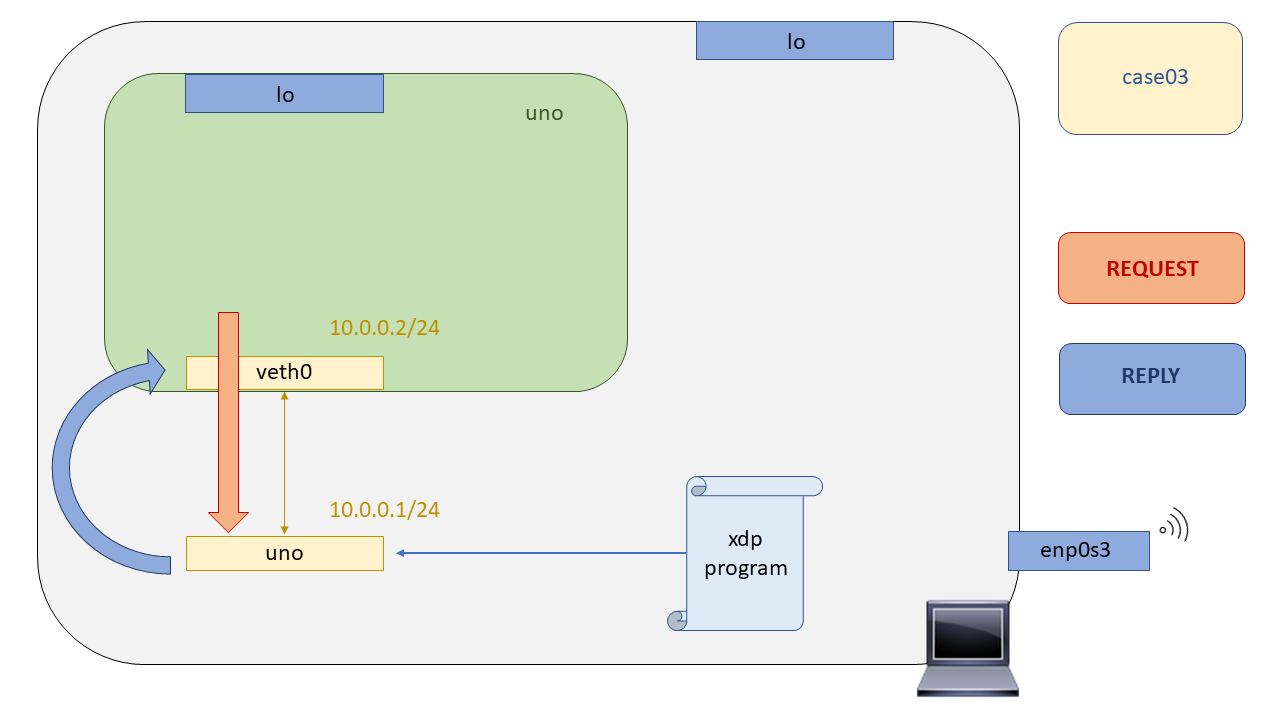
\includegraphics[width=16cm]{archivos/img/dev/xdp/case03/scenario.png}
    \caption{Escenario cableado del Case03 - XDP}
    \label{fig:case03_xdp_ether_scenario}
\end{figure}


\vspace{0.7cm}
\textbf{Carga del programa XDP}\\
\par
Una vez que se tiene el escenario levantado y el programa \gls{xdp} compilado, se procederá a cargarlo en el Kernel. Para más información sobre el programa xdp\_loader, qué aporta la librería libbpf, o por que no se hace uso de la herramienta iproute2 para cargar los programas \gls{xdp} en el Kernel,  se recomienda regresar al case01 (\ref{xdp_ether_case01})  donde se intenta abordar todas estas cuestiones. De forma adicional, es interesante comentar que se va hacer uso del módulo \textbf{netns} de la herramienta iproute2, si tiene alguna duda sobre dicho módulo le recomendamos que consulte su \textit{man-page} o vuelva al case02 (\ref{xdp_ether_case02}) donde se hace una pequeña introducción sobre éste, y su funcionamiento básico para ejecutar comandos ``dentro" de una \textit{Network Namespace}.

\begin{lstlisting}[language= bash, style=Consola, caption={Carga del programa XDP - Case03},label=code:case03_xdp_ether_load]
    # Anclamos el programa XDP (xdp_pass) en la interfaz veth0, perteneciente a la Network Namespace "uno" 
    sudo ip netns exec uno ./xdp_loader -d veth0 -F --progsec xdp_pass
    
    # Anclamos el programa XDP en la interfaz uno, perteneciente a la Network Namespace por defecto
    sudo ./xdp_loader -d uno -F --progsec xdp_case03
\end{lstlisting}
\vspace{0.5cm}

En este caso de uso se anclará el programa \gls{xdp} a validar en la \gls{veth} exterior, por lo que las pruebas vendrán inducidas desde ``dentro" de la \textit{Network Namespace} \texttt{uno}. Para anclar el programa se ha hecho uso de nuevo del programa xdp\_loader. Es importante señalar que se ha tenido que anclar un \textit{dummy program} que permite pasar todos los paquetes a la \gls{veth} destino, esta es una limitación propia por trabajar con \gls{veth}s y \gls{xdp}, de momento se trata de una limitación de implementación, pero puede que a un corto plazo esta limitación se vea ya superada. \\
\par
Para más información sobre esta limitación recomendamos ver la charla de la Netdev llamada ``\textit{\gls{veth}: \gls{xdp} for containers}"\footnote{\url{https://netdevconf.info/0x13/session.html?talk-veth-xdp}} donde explican con un mayor detalle la misma, cómo abordarla y por qué está inducida.

\vspace{0.5cm}
\textbf{Comprobación del funcionamiento}\\
\par

La comprobación del funcionamiento del programa \gls{xdp} anclado a la interfaz \texttt{uno} se llevará a cabo generando pings desde ``dentro" la \textit{Network Namespace} \texttt{uno} hacia afuera. De esta forma la interfaz \texttt{uno} los filtrará, analizará y generará una respuesta. \\
\par
El funcionamiento del programa xdp\_stats es muy simple, ya que desde el programa anclado en el Kernel se genera un mapa \gls{bpf} del tipo clave-valor, donde las claves son los distintos códigos de retorno y los valores son contadores. Después, desde el espacio de usuario el programa xdp\_stats, sabiendo el nombre del mapa \gls{bpf}, y dónde se almacena, va a buscarlo. Para ello, abre el descriptor de archivo asociado a ese mapa almacenado en el path \texttt{/sys/fs/bpf/}. Una vez que tiene abierto el descriptor de archivo, este irá leyendo por clave del mapa todas las estadísticas sobre los códigos de retorno de forma periódica.


\begin{figure}[ht]
    \centering
    \begin{subfigure}[b]{\textwidth}
    	\centering
        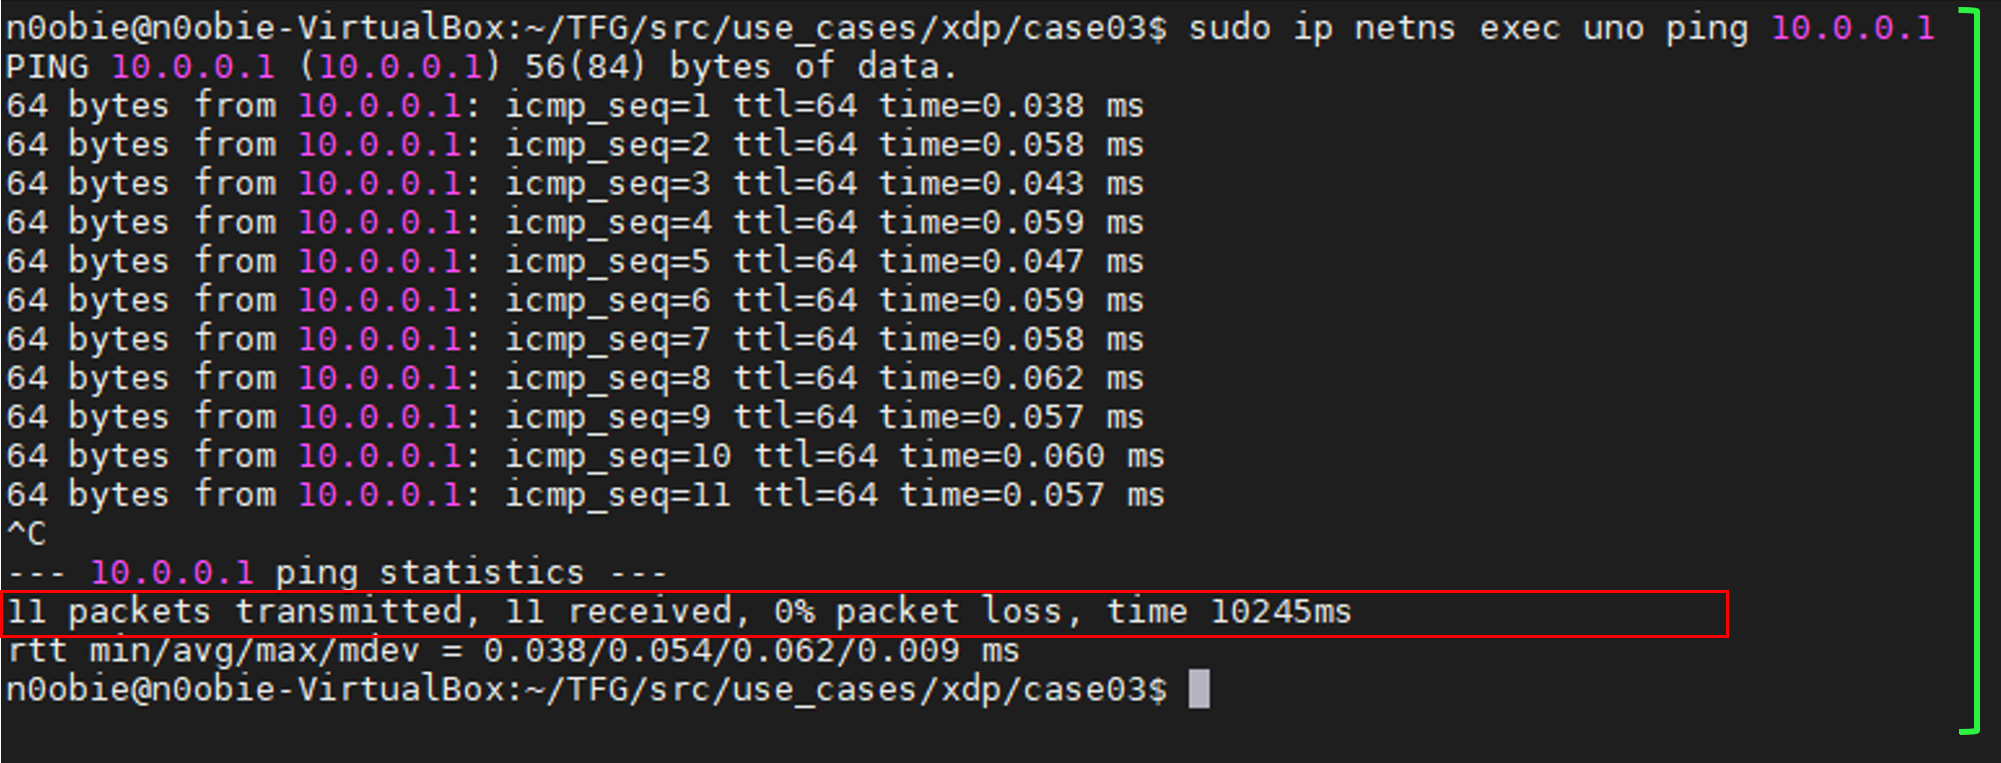
\includegraphics[width=12cm]{archivos/img/dev/xdp/case03/demo_case03_2_edited.png}
        \caption{Ejecución de ping hacia la interfaz con el programa XDP}
        \label{fig:case03_xdp_ether_func_ping}
    \end{subfigure}
    \par\bigskip
    \begin{subfigure}[b]{\textwidth}
    	\centering
        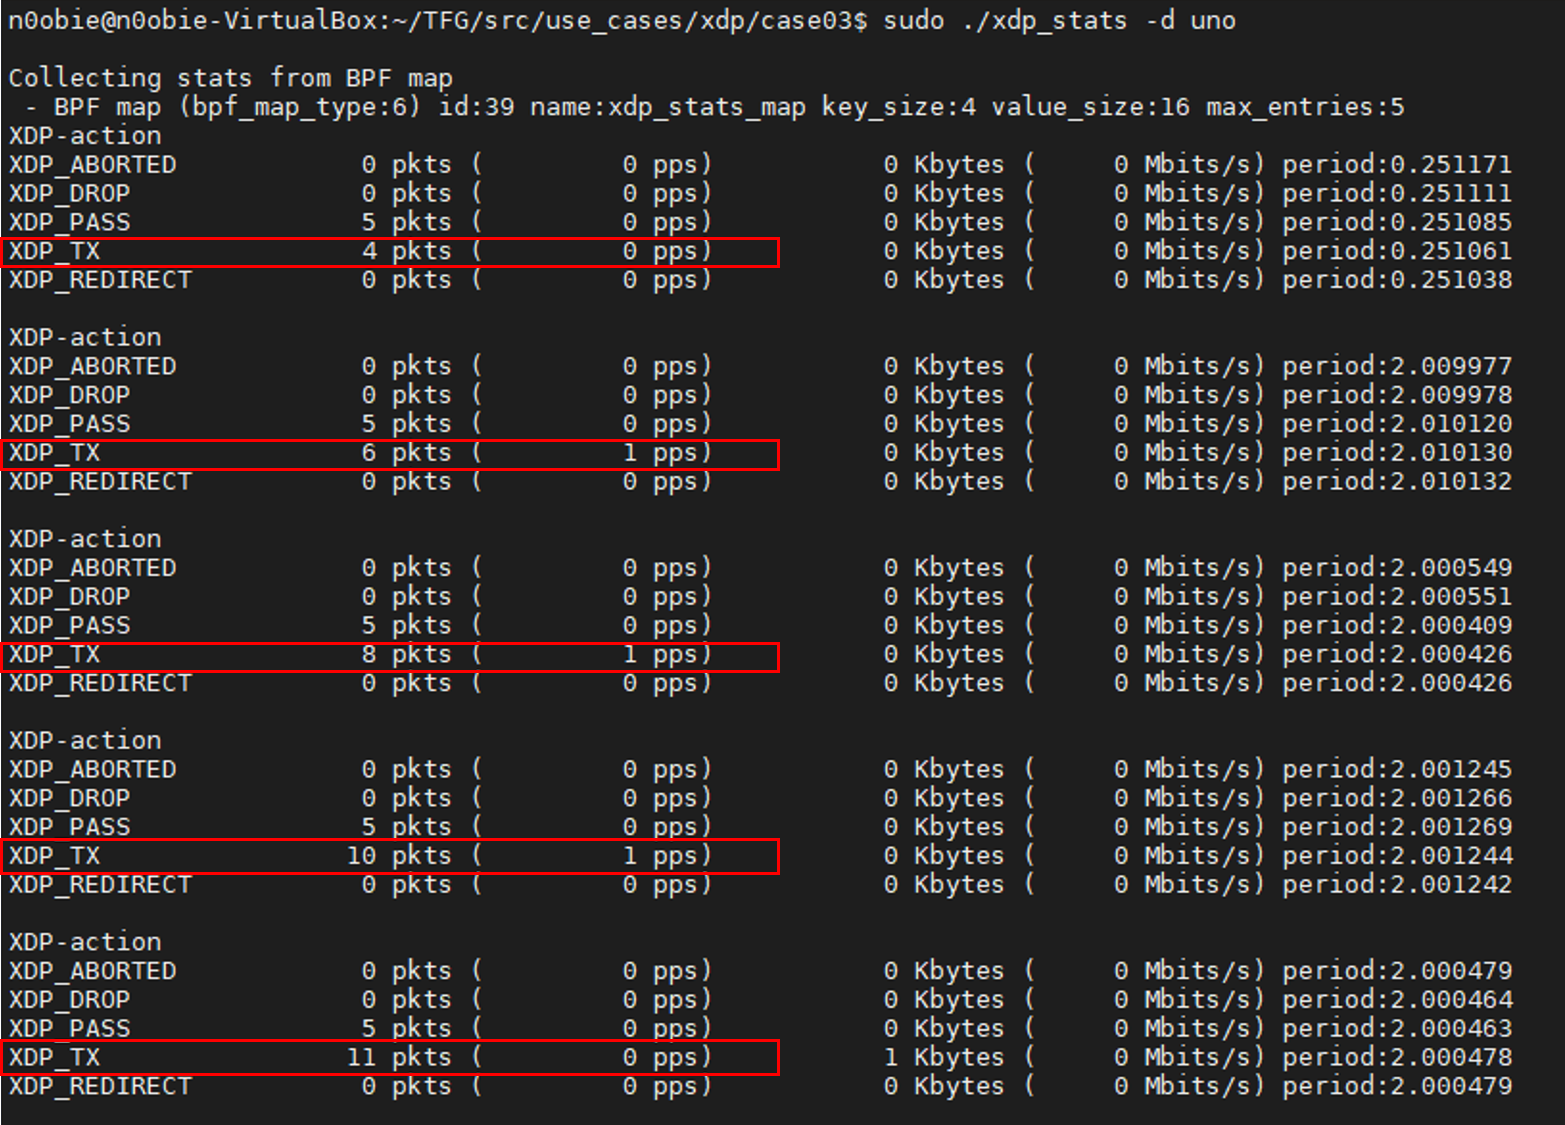
\includegraphics[width=11cm]{archivos/img/dev/xdp/case03/demo_case03_3_edited.png}
        \caption{Estadísticas de los códigos de retorno XDP}
        \label{fig:case03_xdp_ether_func_stats}
    \end{subfigure}
    \caption{Comprobación de funcionamiento del Case03 - XDP}
    \label{fig:case03_xdp_ether_func1}
\end{figure}

Si todo funciona correctamente se debería ver como los códigos de retorno mayormente empleados son los de \texttt{XDP\_TX} siempre y cuando no se haya detenido el ping  desde dentro de la \textit{Network Namespace}. Como se puede apreciar en la figura \ref{fig:case03_xdp_ether_func1}, el ping \fcolorbox{black}{green}{\rule{0pt}{2.5pt}\rule{2.5pt}{0pt}}\hspace{1mm} está siendo contestado correctamente por el programa \gls{xdp} dado que los códigos \texttt{XDP\_TX} van aumentando.\\
\par
De forma adicional, se va a comprobar cómo todos los pings que se manden desde dentro de la \textit{Network Namespace} \texttt{uno} serán contestados. Esto es así, ya que el programa \gls{xdp}, contestará todos los \texttt{ECHO-REQUEST} que le lleguen independientemente de si van dirigidos a él. En la figura \ref{fig:case03_xdp_ether_func2} se puede ver cómo funciona un ping \fcolorbox{black}{orange}{\rule{0pt}{2.5pt}\rule{2.5pt}{0pt}}\hspace{1mm} a una máquina inexistente. Para ello, se ha tenido que añadir una MAC inventada en la tabla ARP asociada a la IP a la cual vamos hacer ping  para que no se iniciara una resolución ARP. En el caso de que se iniciara una resolución ARP, el ping estaría bloqueado a la espera de completar una resolución ARP sobre una máquina inexistente. 

\begin{figure}[h]
    \centering
    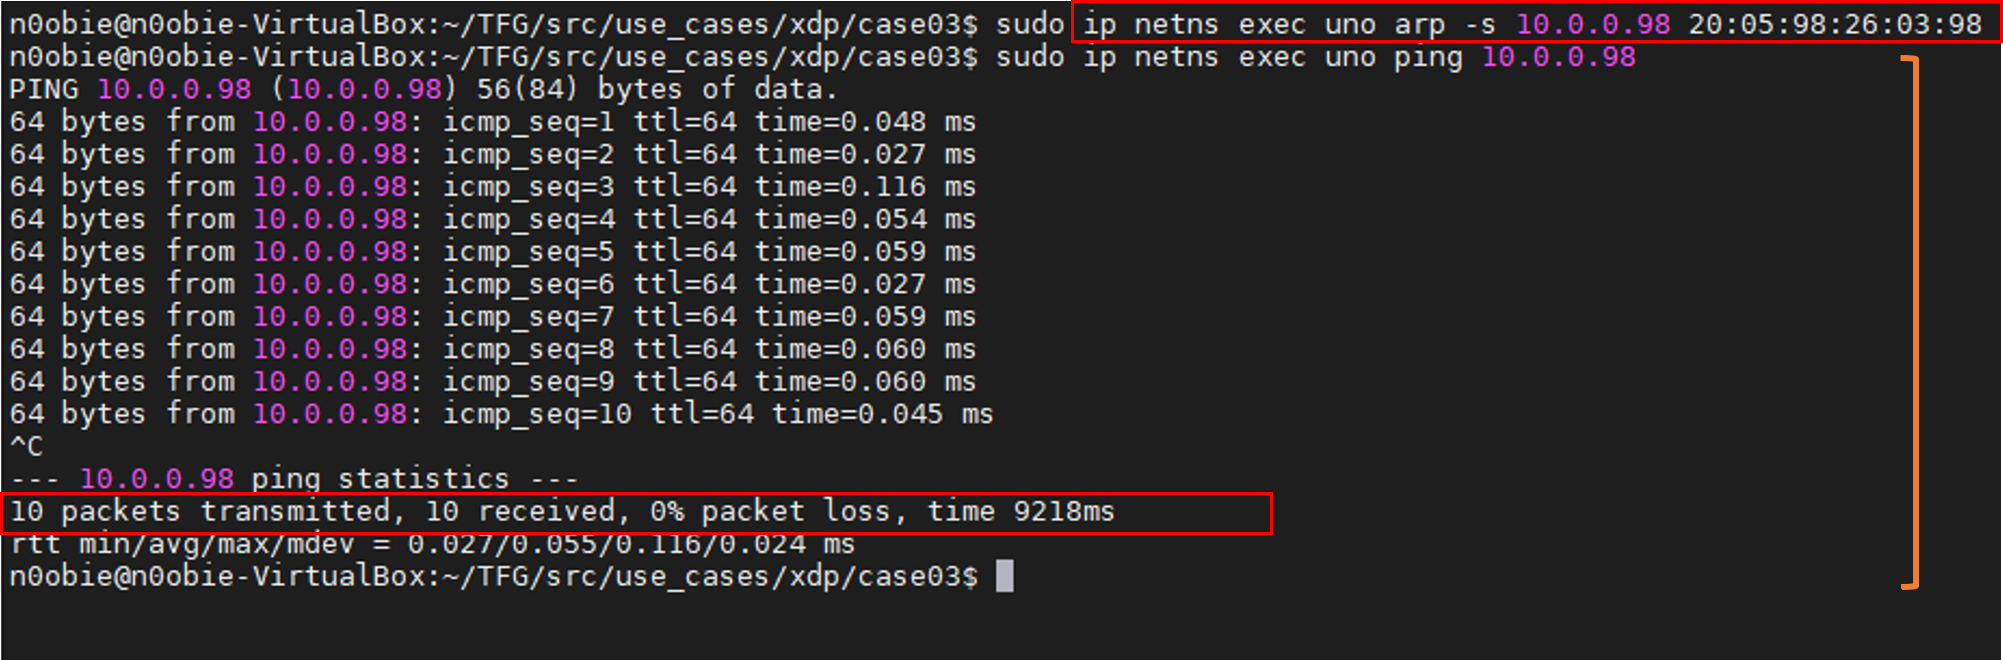
\includegraphics[width=14cm]{archivos/img/dev/xdp/case03/demo_case03_4_edited.png}
    \caption{Ping a máquina inexistente - XDP}
    \label{fig:case03_xdp_ether_func2}
\end{figure}
